% Figure stylisée — Feigenbaum & Gross (2024)
% Représentation schématique de l'event study, pas reproduction des données
\begin{figure}[htbp]
\centering
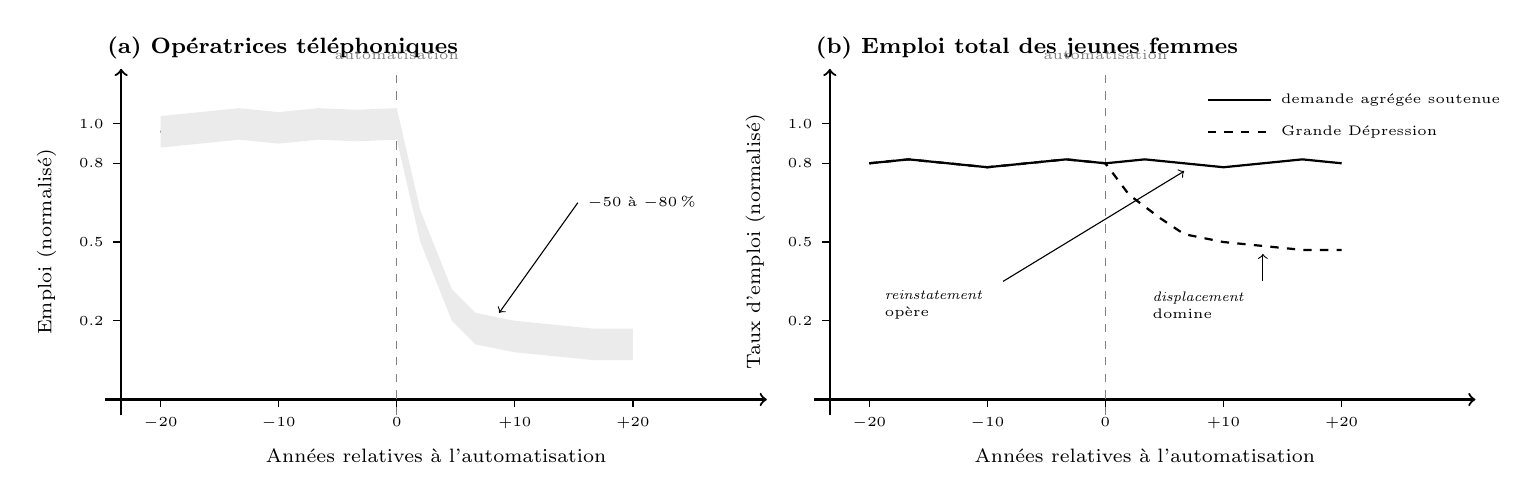
\begin{tikzpicture}
\begin{scope}[xshift=0cm]
  % Panel (a) — Opératrices
  \node[anchor=south west, font=\footnotesize\bfseries] at (-0.3,4.2) {(a) Opératrices téléphoniques};
  
  % Axes
  \draw[->, thick] (-0.2,0) -- (8.2,0) node[right, font=\scriptsize] {};
  \draw[->, thick] (0,-0.2) -- (0,4.2);
  
  % Labels axes
  \node[font=\scriptsize, below] at (4,-0.5) {Années relatives à l'automatisation};
  \node[font=\scriptsize, rotate=90, above] at (-0.7,2) {Emploi (normalisé)};
  
  % Tick marks x
  \foreach \x/\lab in {0.5/$-20$, 2/$-10$, 3.5/$0$, 5/$+10$, 6.5/$+20$} {
    \draw (\x,0) -- (\x,-0.1) node[below, font=\tiny] {\lab};
  }
  
  % Tick marks y
  \draw (0,1) -- (-0.1,1) node[left, font=\tiny] {0.2};
  \draw (0,2) -- (-0.1,2) node[left, font=\tiny] {0.5};
  \draw (0,3) -- (-0.1,3) node[left, font=\tiny] {0.8};
  \draw (0,3.5) -- (-0.1,3.5) node[left, font=\tiny] {1.0};
  
  % Cutover line
  \draw[dashed, gray] (3.5,-0.2) -- (3.5,4.2);
  \node[font=\tiny, gray, above] at (3.5,4.2) {automatisation};
  
  % Pre-cutover: flat at ~3.5
  \draw[thick, black] (0.5,3.4) -- (1,3.45) -- (1.5,3.5) -- (2,3.45) -- (2.5,3.5) -- (3,3.48) -- (3.5,3.5);
  
  % Post-cutover: sharp drop to ~1, then stays low
  \draw[thick, black] (3.5,3.5) -- (3.8,2.2) -- (4.2,1.2) -- (4.5,0.9) -- (5,0.8) -- (5.5,0.75) -- (6,0.7) -- (6.5,0.7);
  
  % Annotation
  \draw[<-, thin] (4.8,1.1) -- (5.8,2.5) node[right, font=\tiny, text width=2cm] {$-50$ à $-80\,\%$};
  
  % Confidence band (very light)
  \fill[black!8] (0.5,3.2) -- (1,3.25) -- (1.5,3.3) -- (2,3.25) -- (2.5,3.3) -- (3,3.28) -- (3.5,3.3) -- (3.5,3.7) -- (3,3.68) -- (2.5,3.7) -- (2,3.65) -- (1.5,3.7) -- (1,3.65) -- (0.5,3.6) -- cycle;
  \fill[black!8] (3.5,3.3) -- (3.8,2.0) -- (4.2,1.0) -- (4.5,0.7) -- (5,0.6) -- (5.5,0.55) -- (6,0.5) -- (6.5,0.5) -- (6.5,0.9) -- (6,0.9) -- (5.5,0.95) -- (5,1.0) -- (4.5,1.1) -- (4.2,1.4) -- (3.8,2.4) -- (3.5,3.7) -- cycle;
\end{scope}

\begin{scope}[xshift=9cm]
  % Panel (b) — Emploi total
  \node[anchor=south west, font=\footnotesize\bfseries] at (-0.3,4.2) {(b) Emploi total des jeunes femmes};
  
  % Axes
  \draw[->, thick] (-0.2,0) -- (8.2,0);
  \draw[->, thick] (0,-0.2) -- (0,4.2);
  
  % Labels
  \node[font=\scriptsize, below] at (4,-0.5) {Années relatives à l'automatisation};
  \node[font=\scriptsize, rotate=90, above] at (-0.7,2) {Taux d'emploi (normalisé)};
  
  % Tick marks x
  \foreach \x/\lab in {0.5/$-20$, 2/$-10$, 3.5/$0$, 5/$+10$, 6.5/$+20$} {
    \draw (\x,0) -- (\x,-0.1) node[below, font=\tiny] {\lab};
  }
  
  % Tick marks y
  \draw (0,1) -- (-0.1,1) node[left, font=\tiny] {0.2};
  \draw (0,2) -- (-0.1,2) node[left, font=\tiny] {0.5};
  \draw (0,3) -- (-0.1,3) node[left, font=\tiny] {0.8};
  \draw (0,3.5) -- (-0.1,3.5) node[left, font=\tiny] {1.0};
  
  % Cutover line
  \draw[dashed, gray] (3.5,-0.2) -- (3.5,4.2);
  \node[font=\tiny, gray, above] at (3.5,4.2) {automatisation};
  
  % Solid line: employment stays flat (normal conditions)
  \draw[thick, black] (0.5,3.0) -- (1,3.05) -- (1.5,3.0) -- (2,2.95) -- (2.5,3.0) -- (3,3.05) -- (3.5,3.0) -- (4,3.05) -- (4.5,3.0) -- (5,2.95) -- (5.5,3.0) -- (6,3.05) -- (6.5,3.0);
  
  % Dashed line: Depression cities — drops after cutover
  \draw[thick, black, dashed] (0.5,3.0) -- (1,3.05) -- (1.5,3.0) -- (2,2.95) -- (2.5,3.0) -- (3,3.05) -- (3.5,3.0) -- (3.8,2.6) -- (4.2,2.3) -- (4.5,2.1) -- (5,2.0) -- (5.5,1.95) -- (6,1.9) -- (6.5,1.9);
  
  % Legend
  \draw[thick, black] (4.8,3.8) -- (5.6,3.8) node[right, font=\tiny] {demande agrégée soutenue};
  \draw[thick, black, dashed] (4.8,3.4) -- (5.6,3.4) node[right, font=\tiny] {Grande Dépression};
  
  % Annotation
  \node[font=\tiny, text width=2.2cm, align=left] at (1.8,1.2) {\emph{reinstatement}\\opère};
  \draw[->, thin] (2.2,1.5) -- (4.5,2.9);
  
  \node[font=\tiny, text width=2.2cm, align=left] at (5.2,1.2) {\emph{displacement}\\domine};
  \draw[->, thin] (5.5,1.5) -- (5.5,1.85);
\end{scope}
\end{tikzpicture}

\caption[Automatisation de la commutation téléphonique~: displacement et reinstatement]{Représentation stylisée du résultat de \textcite{feigenbaum_answering_2024}. Panel~(a)~: l'emploi des opératrices chute de 50 à 80\,\% après l'automatisation. Panel~(b)~: le taux d'emploi total des jeunes femmes reste stable dans les villes à demande agrégée soutenue (trait plein), mais baisse dans les villes frappées par la Grande Dépression (trait pointillé). La compensation opère entre cohortes, pas au sein d'une cohorte~: les incumbents perdent~; les entrantes se réallouent. Source~: construction de l'auteur d'après \textcite{feigenbaum_answering_2024}.}
\label{fig:feigenbaum-stylized}
\end{figure}
